\documentclass{article}
\usepackage[utf8]{inputenc}
\usepackage[nottoc]{tocbibind}
\usepackage{ amssymb }
\usepackage{enumerate}
\usepackage{graphicx}
\title{Contrary-to-Duty Paradoxes\\{\normalsize  \underline{BACHELOR-SEMINAR INFORMATIK  (WS 20/21)}}}
\author{Yingqin Fu 702065 Markus Davydov 690672 }
\date{December 2020}

\begin{document}
\maketitle

\tableofcontents
\section*{Abstract}
We will summerize the first problem of Deontic Logic ,the so-called Contrary-to-duty (CTD) in this paper.A contrary-to-duty obligation tells us,what we ougt to do if something is forbidden.Which is very important in our moral and legal thinking.So we want to discuss the problem with different deontic logic systems,and try to find a way to explain it.\\
Keywords:contrary-to-duty Paradoxes(CTD),Chisholm’s paradox,Standard deontic logic(SDL)
\section*{Introduction}
What is contrary-to-duty obligation?And why is it a Paradoxes? A contrary-to-duty obligation is an obligation telling us what ought to be the case if something forbidden is true. Here are some examples of sentences that often express such obligations: ‘If she is guilty, she should confess’, ‘If he has hurt his friend, he should apologise to her’, ‘If you are not going to keep your promise to him, you ought to call him’, ‘If the books are not returned by the due date, you must pay a fine’. In this paper we will summarize the first part of the paper"Multiagent Deontic Logic and its Challenges from a Normative Systems Perspective "\cite{1} 
\section{ Chisholm's paradox}
First of all,We are going to introduce first the so-called Chisholm's paradox\cite{2},which is know as one of the earliest CTD paradox.
Chisholm's paradox consists of the following four sentences:
\begin{enumerate}
\item  It ought to be that a certain man go to the assistance of his neighbours.
\item  It ought to be that if he does go, he tell them he is coming.
\item If he does not go then he ought not to tell them he is coming.
\item He does not go.
\end{enumerate}
Chisholm’s paradox is a contrary-to-duty paradox, since it contains both a primary obligation to go, and a secondary obligation not to tell if the agent does not go.Yet intuitively the natural-language expressions
that make up the paradox are consistent and independent from each other: this is
why it is called a paradox.\\
There are also various kinds of scenarios which are similar to Chisholm’s scenario.For example, van Benthem, Grossi and Liu \cite{3} givethe following example, in the formulation proposed by Åqvist:\\
\begin{description}
\item[(1)] It ought to be that Smith refrains from robbing Jones.
\item[(2)] Smith robs Jones.
\item[(3)]If Smith robs Jones, he ought to be punished for robbery.
\item[(4)]It ought to be that if Smith refrains from robbing Jones he is not punished
for robbery.
\end{description}



Contrary-to-duty obligations turn up in discussions concerning guilt, blame, restoration, reparation, confession, punishment, repentance, retributive justice, compensation, apologies, damage control, etc. Therefore, they are important in our moral and legal thinking. The rationale of a contrary-to-duty obligation is the fact that most of us do neglect our primary duties from time to time and yet it is reasonable to believe that we should make the best of a bad situation, or at least that it matters what we do when this is the case. Everyone needs to find a way,that tells us what to do, when we don't finish the things we ought to do.In this paper,we will try to find a adequate formal representation of such obligations.
\section{Monadic deontic logic}
Traditional or ‘standard’ deontic logic, often referred to as SDL, was introduced by Von Wright\cite{4}.SDL regards as the most basic system of deontic logic,but also may have the most drawback.In this section,we try to analyze the Chisholm’s paradox with the basic SDL system.
\subsection{language}
$\varphi :=\perp | p |\neg \varphi |(\varphi \wedge \varphi)|\bigcirc\varphi|\square\varphi $\\
Given two arbitrary formulas $\psi$  and $\varphi$, then\\
$\perp$:the empty symbol\\
$\neg$ $\varphi$: classical negation\\
$\varphi \vee  \psi $: classical disjunction\\
$\bigcirc \varphi $: $\varphi$ is obligatory\\
$ \neg \bigcirc\neg\varphi$: $ \varphi$ is forbidden\\
$ \square\varphi$: $\varphi$ is necessary
\subsection{Semantics}
\begin{description}
\item[$\bullet$ ] let $\nu$ be a valuation function on AP
\item[$\bullet $]  let M = (W, R) A kripke model with on worlds W related via R : W × W
\item[$\bullet $]  "M,s $ \vDash \varphi$" is read a state s satisfies $\varphi$ in the Model M,we define the satisfaction relation M,s $ \vDash \varphi$ by induction on $\varphi$ using the clauses:
\begin{description}
\item[$\bullet$ ]M, s $ \vDash $ p iff s $\in$ $\nu$  (p)
\item[$\bullet$ ]M, s $ \vDash $ $\neg \varphi$ iff not M, s $ \vDash $ $\varphi$
\item[$\bullet$ ]M, s $ \vDash $ $(\varphi\land\psi )$ iff M,s $ \vDash \varphi$ and  M,s $ \vDash \psi$
\item[$\bullet$ ]M, s $ \vDash  \bigcirc\varphi$ iff for all t,if Rst then M, t$\vDash \varphi$
\item[$\bullet$ ]M, s $ \vDash  \square\varphi$ iff for all t $\in$ W, M, t $\vDash \varphi$
\end{description}
\end{description}
Axioms for Standard Deontic Logic:
\begin{enumerate}
\item Taut: All tautologies are Well formed formulas of the language.
\item  $Axiom K: O(p \to q) \to (O(p) \to O(q)) $
\item $ Axiom D: O(p) \to \neg O(\neg p)$
\item $Modus Ponens: ((p \to q) \land p) \to q $
\item $ Necessity: p \to O(p)$
\end{enumerate}
\subsection{Limitations}
Now we focus on the Chisholm'paradox with the Monadic deontic logic.
We can describe the four sentences of Chisholm'paradox with the Monadic Deontic logic(h:= he goes to help his neighbours; t:=he tell them),we have four different ways to describe them:
\begin{enumerate}
\item $(1)O(h);(2)O(h\to t);(3)O(\neg h\to \neg t);(4) \neg h$
\item $(1)O(h);(2)O(h \to t);(3) \neg h \to O (\neg t); (4) \neg h$
\item $(1)O(h);(2)h\to O(t);(3)\neg h \to O(\neg t) ;(4)\neg h $
\item $ (1)O(h);(2)h\to O(t)(3)O(\neg h\to \neg t)(4)\neg h$
\end{enumerate}
Now we foucs on the above-mentioned four SDL descriptions:
\begin{enumerate}
\item From (4) and Axiom 5 ,we have $O(\neg h) $ ;From (1) and (2),we have O(t);From $O(\neg h)$ and (3),we have $ O(\neg t)$. Obviously,O(t) $\wedge$ $O(\neg t)$ is paradox.
\item From (3) and (4) with Axiom MP,we have $O(\neg t)$;From (2) and Axiom K,we have $O(h)\to O(t) $;which with (1) and Axiom MP,we have O(t)
\item We know that,$ \neg h \to (h \to O(t))$ is Taut,which with (4) can we have $ h \to O(t)$.it is identical to (2).Hence,it's redundant.
\item It's redundant with the same reason of 3.
\end{enumerate}
Hence,we can conclude,that under the Monadic Deontic Logic(SDL) the CTD is
\textbf{inconsistent} and \textbf{redundant}.Something must be wrong with our formalisation, with SDL or with our intuitions. In a nutshell, this puzzle is the contrary-to-duty
(obligation) paradox.\\

So how can we overcome the limitation of SDL?Can we extend the semantics of SDL?For example,one can add distinct modal operators for primary and secondary obligations, where a secondary obligation is a kind of reparational obligation.So with the Chisholm’s paradox,we regard 1 and 2 as primary obligation(he ought to go),3 as secondary obligation(he ought to tell his neighbours).So the sentences are now:
\begin{description}
\item[(1)] $\bigcirc_{1} h$
\item[(2)]$\bigcirc_{1}$ ($h \to t $)
\item[(3)]$\neg h \to \bigcirc_ {2} (\neg t)$
\item[(4)]$\neg h$
\end{description}
From 1-4 we can derive only $\bigcirc_{1} \neg t \wedge \bigcirc_{2} t$,which is consistent.\\
Seems like we find a good way to solve the limitation of SDL.However,it may not always be easy to distinguish primary from secondary obligations, because it may depend on the context whether an obligation is primary or secondary. It's not easy for us to describe the ideal world with this solution. 
\section{Dyadic deontic logic}
Dyadic deontic logic(or Dyadic Standard Deontic Logic ) is the logic for reasoning with dyadic obligations (“it ought to be the case that ... if it is the case that ...").The language is extended with dyadic operators 
 $\bigcirc(p|q)$, which is true iff the preferred q worlds satisfy p. The class of logics is called Dyadic ‘Standard’ Deontic Logic or DSDL. The notation is inspired by the representation of conditional probability.
In this section, we will reasoning CTD with DDL.
\subsection{Language}
$\varphi := \perp | p | \neg \varphi |(\varphi \wedge \varphi)|\square \varphi |\bigcirc(\varphi|\varphi)$\\
Given two arbitrary formulas $\psi$  and $\varphi$, then\\
$\perp$:the empty symbol\\
$\neg$ $\varphi$: classical negation\\
$\varphi \vee  \psi $: classical disjunction\\
$\bigcirc \varphi $: $\varphi$ is obligatory\\
$ \neg \bigcirc\neg\varphi$: $ \varphi$ is forbidden\\
$ \square\varphi$: $\varphi$ is necessary\\
$\bigcirc(\varphi\mid\psi$): It ought to be $\varphi$,given $\psi$\\
$P(\varphi\mid\psi) $:$\varphi$ is permitted,given $\psi$,as an abbreviation of $\neg\bigcirc(\neg\varphi\mid\psi)$\\
$\lozenge(\varphi)$:possibly $\varphi$,as an abbreviation of $\neg\square\neg\varphi$\\
\subsection{Semantics}
A preference model M = (W, $\geq$, V ) is a structure where:
\begin{description}
\item[$\bullet$ ] W is a nonempty set of worlds.
\item[$\bullet $] $ \geq$ is a reflexive, transitive relation over W satisfying the following limitedness requirement: if $\|\varphi\| \neq \emptyset, then {x\in\|\varphi\| : (\forall y \in \|\varphi\|)x\geq y} \neq \emptyset. Here\|\varphi\| = {x \in W : M, x\vDash \varphi}.$
\item[$\bullet$]V is a standard propositional valuation such that for every propositional letter p, V (p) $\subseteq$ W.
\begin{description}
\item[$\bullet$ ]M, s $ \vDash $ p iff s $\in$ $\nu$  (p)
\item[$\bullet$ ]M, s $ \vDash $ $\neg \varphi$ iff not M, s $ \vDash $ $\varphi$
\item[$\bullet$ ]M, s $ \vDash $ $(\varphi\land\psi )$ iff M,s $ \vDash \varphi$ and  M,s $ \vDash \psi$
\item[$\bullet$ ]M, s $ \vDash  \bigcirc(\psi\mid\varphi) iff \forall t(((M, t \vDash \varphi)\with\forall u(M, u \vDash \varphi) \Rightarrow t \geq u) \Rightarrow M, t \vDash \psi)$
\item[$\bullet$ ]M, s $ \vDash  \square\varphi$ iff for all t $\in$ W, M, t $\vDash \varphi$
\end{description}
\end{description}
\subsection{Limitations}
The following example is a variant of the scenario originally phrased by Chisholm in 1963. There is widespread agreement in the literature that, from the intuitive point of view, this set of sentences is consistent, and its members are logically independent of each other.
\begin{description}
\item[A]It ought to be that Jones does not eat fast food for dinner.
\item[B]It ought to be that if Jones does not eat fast food for dinner, then he does not go to McDonald’s.
\item[C] If Jones eats fast food for dinner, then he ought to go to McDonald’s.
\item[D]Jones eats fast food for dinner.
\end{description}
We try to reasoning the above-mentioned sentences with DSDL(f:Jones eats fast food for dinner;m:he goes to McDonald’s ):
\begin{description}
\item[A]$\bigcirc \neg f$
\item[B]$\bigcirc(\neg m \mid \neg f)$
\item[C]$\bigcirc(m\mid f)$
\item[D]f
\end{description}
the dyadic representation A - D highlights the dilemma between factual detachment (FD) and deontic detachment (DD)
\begin{description}
\item[Axiom FD]$\bigcirc(m\mid f),f \Rightarrow \bigcirc m$\\
\item[Axiom DD]$\bigcirc(\neg m \mid \neg f), \bigcirc\neg f \Rightarrow \bigcirc\neg m$\\
\end{description}

From A and B with(axiom DD) ,we have $\bigcirc\neg  m$;From C and D(axiom FD),we have $\bigcirc m$ , as we simply derive a dilemma:$\bigcirc\neg m\wedge\bigcirc m$\\
Hence,there is also something wrong with the DSDL,when we try to reasoning CTD paradox.\\
The main drawback of DSDL is that in a monotonic setting, we cannot detach
the obligation $\bigcirc m$ from the four sentences.

\section{Input/Output logic}
Input/output logic\cite{5} ,which  is a non classical logic,takes its origin in the study of conditional norms. These may express desired features of a situation, obligations under some legal, moral or practical code, goals, contingency plans, advice, etc. Typically they may be expressed in terms like: In such-and-such a situation, so-and-so should be the case, or …should be brought about, or …should be worked towards, or …should be followed – these locutions corresponding roughly to the kinds of norm mentioned.
 Input/output logic may be seen as an attempt to extract the essential mathematical structure behind the reconstruction of deontic logic.\\
 \subsection{Definition}
   Technically, a normative code is seen as a set G of conditional norms, i.e. a set of such ordered pairs (a,x). For each such pair, the body a is thought of as an input, representing some condition or situation, and the head x is thought of as an output, representing what the norm tells us to be desirable, obligatory or whatever in that situation.
\begin{figure*}[hb]
\centering
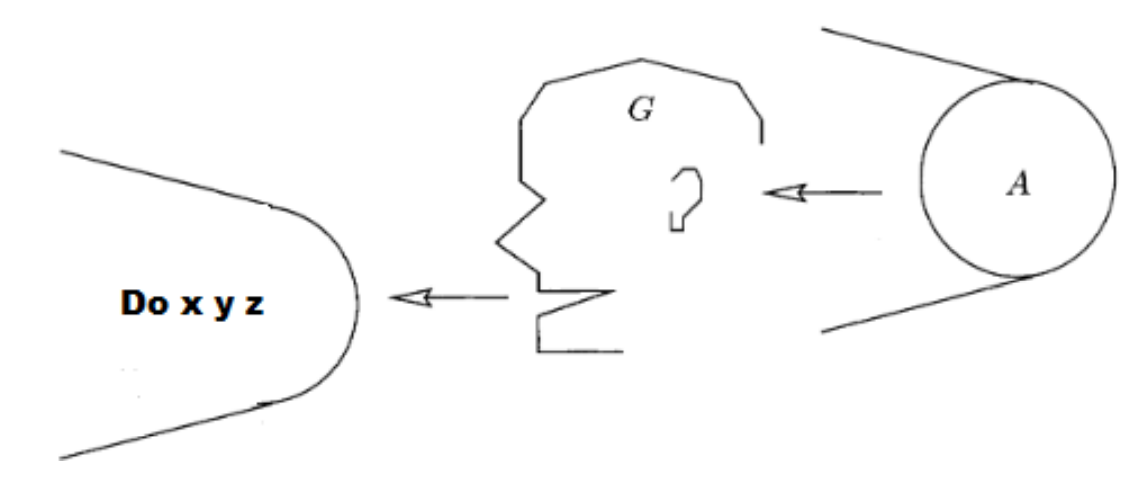
\includegraphics[scale=0.45]{input_output.png}
\label{fig_framework}
\end{figure*}\\
Cn(A) denotes the set of logical consequences of A in classical propositional
logic.It returns the set of all provable propositional formulae provable assuming the fact in A( the set of answers of a set of inputs).For example,\\
A= \{ x, y\} then Cn(A) = \{x, y, x $\vee $y, x $\wedge$ y $\vee$ . . . \}\\
The simplest kind of input/output operation is depicted in Figure 1. A
set A of propositions serves as explicit input, which is prepared by being expanded to its classical closure Cn(A). This is then passed into the ‘black box’ or ‘transformer’ G, which delivers the corresponding immediate output G(Cn(A)) = \{x: for some a $\in$ Cn(A), (a,x) $\in$ G\} Finally, this is expanded by classical closure again into the full output $out_{1}$(G,A) = Cn(G(Cn(A))). We call this simple-minded output.\\

\begin{figure*}[hb]
\centering
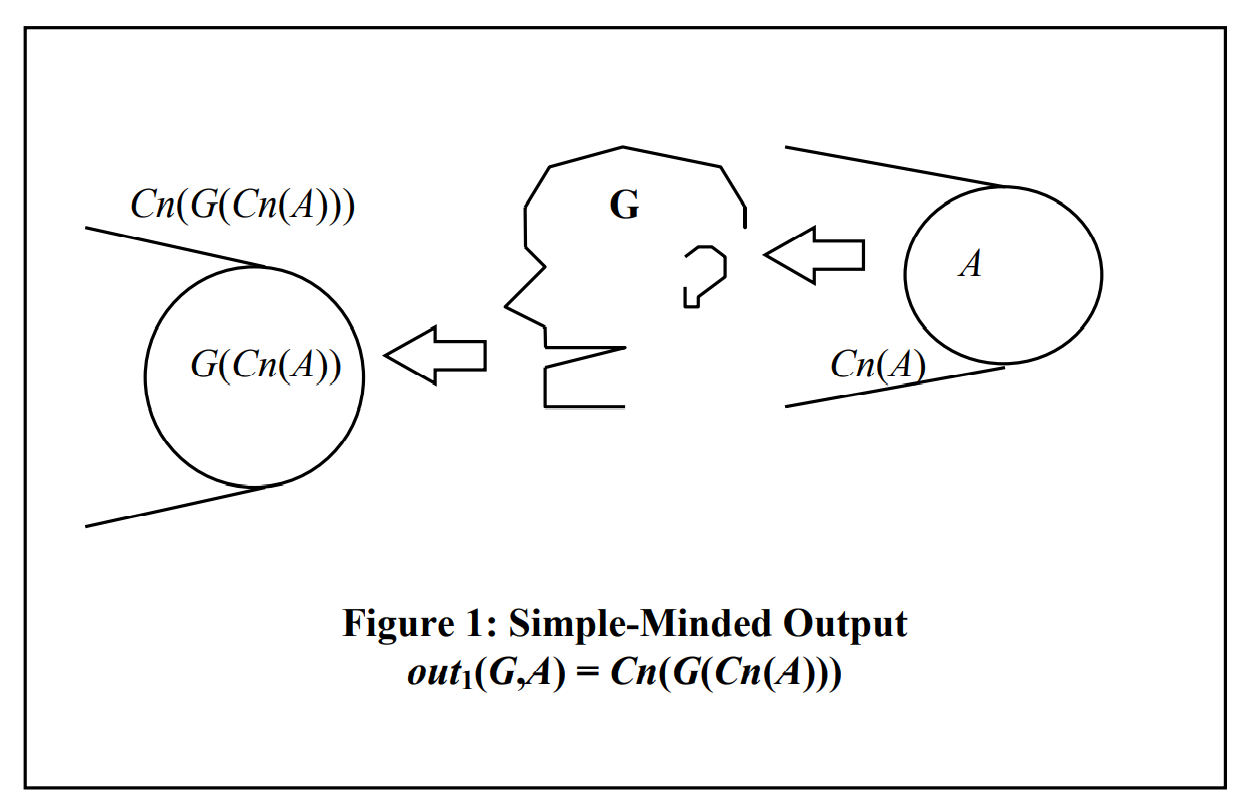
\includegraphics[scale=0.4]{simple_minded.png}

\label{fig_framework}
\end{figure*}
What's more,there are 5  rules in I/O logic:
\begin{description}
\item[$\bullet$] Strengthening Input (SI): From (a,x) to (b,x) whenever a $\in$ Cn(b)
\item[$\bullet$] Conjoining Output (AND): From (a,x), (a,y) to (a,x$\wedge$y)
\item[$\bullet$] Weakening Output (WO): From (a,x) to (a,y) whenever y $\in$ Cn(x).
\item[$\bullet$] Disjoining input (OR): From (a,x), (b,x) to (a$\vee$b,x)
\item[$\bullet$] Cumulative transitivity (CT): From (a,x), (a$\wedge$x,y) to (a,y).
\end{description}
There are also four very natural systems of input/output, which are labelled as follows: 
\begin{description}
\item[$\bullet$]simple-minded alias $out_{1}$ (as above)
\item[$\bullet$]basic (simple-minded plus input disjunction: $out_{2}$)
\item[$\bullet$]reusable (simple-minded plus reusability: $out_{3}$)
\item[$\bullet$]reusable basic alias $out_{4}$
\end{description}
For example,$out_{4}$ can be given by Figure 2.\\
\newpage
\begin{figure*}[hb]
\centering
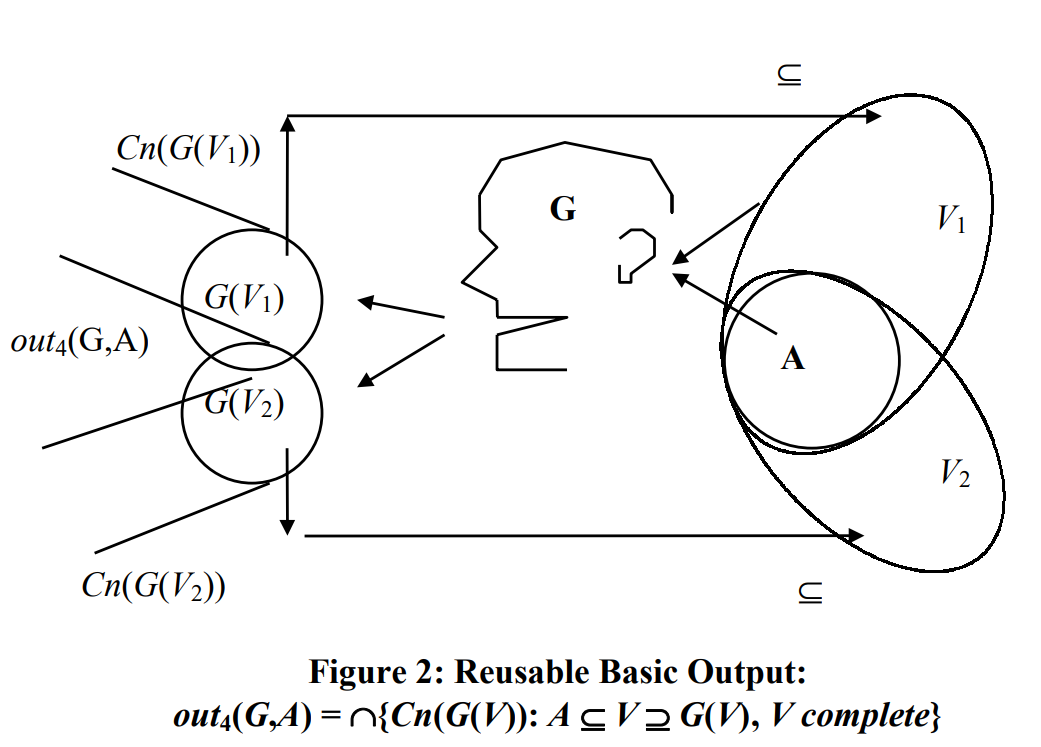
\includegraphics[scale=0.5]{out4.png}

\label{fig_framework}
\end{figure*}
After the simple introduction of Input/Output logic,we reconsider our topic,the Contrary to duty obligations.
\subsection{Contrary to duty reasoning}
Like every other approach to deontic logic, input/output logic must face the problem of accounting adequately for the behaviour of  ‘contrary-to-duty’ norms. The problem may be stated thus: given a set of norms to be applied, how
should we determine which obligations are operative in a situation that already
violates some among them. It appears that input/output logic provides a convenient platform for dealing with this problem by imposing consistency constraints on the generation of output.
\subsubsection{Definition(Maxfamilies)}
Let G be a set of conditional norms and A and C two sets of propositional formulas.\\
Then maxfamily(G, A, C) is the set of maximal
subsets H $\subseteq$ G such that out(H, A) $\cup$ C is consistent.(which means,out(H,A)) is consistent with C.)\\
For a possible solution to Chisholm’s paradox, consider the following output operation $out^{\cap}$:\\
$out^{\cap}(G, A) = \cap
\{out(H, A) | H \in maxfamily(G, A, A)\}
$
\subsubsection{Contrary to duty reasoning}
Let G a "Chisholm norm set";\\
x means the norm that a man goes to the assistence of his neighbors;\\
z means the norm that he tells them he is coming\\
\begin{description}
\item[$\bullet$]G=$\{(\top ,x),(x,z),(\neg x,\neg z)  \}$\\
 $(\top ,x)$ means the norm that the man must go to the assistance of his neighbors;$(x,z)$means the norm that it ought to be that if he goes he ought to tell them he is coming;$(\neg x,\neg z)$ means that the norm that if he does not go he ought not to tell them he is coming.
 \item[$\bullet$] $A=\{ \neg x \}$
 \item[$\bullet$] We have H $\in out_{1}(G,A)=\{x,\neg z\}$ ,which is inconsistent with A because of $\top$
 \item[$\bullet$] We have  H = maxfamily(G,A,A)=$ \{ G\setminus \{(\top,x) \}\}=\{\{(x,z),(\neg x,\neg z)   \}\} $
 \item[$\bullet$] out(H,A)=$\neg z$,which is consistent with A
 \item[$\bullet$]$out^{\cap}(G,A)=Cn(\neg z)$ ,which means the form that the man must not tell his neighbors he is coming
\end{description}
Hence,the Input/output logic is able to handle the CTD paradox,which is a proposed solution of it.
\section{Counterfactual Deontic Logic}
  Counterfactual Deontic Logic\cite{6},which is introduced by Rönnedal in 2016.The Counterfactual Deontic Logic combine the Counterfactual Logic with Deontic Logic.It aims at the relationship between the obligation and time.
\subsection{Definition}
\begin{description}
\item[$\bullet$]$A\square \rightarrow B$ is often read ‘If A were the case, then B would be the case’
\item[$\bullet$]R is a temporal operator; ‘$Rt_{1}$A’ says that it is realised at time t1 (it is true at t1) that A
\end{description}
\subsection{ Contrary to duty reasoning}
Consider the following sentences about Contrary to duty paradox
\begin{description}
\item[1] (On Monday it is true that) You ought to keep your promise (and see your friend on Friday).
\item[2] (On Monday it is true that) It ought to be that if you keep your promise, you do not apologise (when you meet your friend on Saturday).
\item[3](On Monday it is true that) If you do not keep your promise (i.e. if you do not see your friend on Friday and help her out), you ought to apologise (when you meet her on Saturday).
\item[4](On Monday it is true that) You do not keep your promise (on Friday).
\end{description}
With the help of Counterfactual Deontic Logic,the four sentences can now be symbolised in the following way:(R is a temporal operator;t1,t2,t3 are the different time;k is keep promise;and a is apologise )
\begin{description}
\item[CF1]$Rt_{1}ORt_{2}k$
\item[CF2]$Rt_{1}O(Rt_{2}k \square \rightarrow Rt_{3}\neg a)$
\item[CF3]$Rt_{1}(Rt_{2}\neg k \square \rightarrow Rt_{2}ORt_{3}a)$
\item[CF4]$Rt_{1}Rt_{2}\neg k$
\end{description}
We can see:
\begin{description}
\item[$\bullet$] CF-CTD is consistent,It does not seem to be possible to deduce any contradiction from the four sentences. Hence, we want our symbolisation of this set to be consistent. In this respect, CF-CTD is an intuitively plausible formalisation of the four sentences.
\item[$\bullet$] CF-CTD is non-redundant.There ist no sentence in this set follows from the rest.

\end{description}
\subsection{Limitations}
The Counterfactual Deontic Logic seems to be a proposed solution of CTD-paradox(at least in our example).However,it also has limitations.\\
\begin{description}
\item[$\bullet$]the Counterfactual Solution cannot Handle Timeless (or Parallel)
Contrary-to-Duty Paradoxes;
\item[$\bullet$]the Counterfactual Solution cannot Solve Beforehand
Contrary-to-Duty Paradoxes
\end{description}

\section{Alternative approaches}
In this section,we summerize easily the other Analyse of other reaserchers.\\

  Carmo and Jones \cite{7} suggest that the representation of the facts is challenging,
instead of the representation of the norms. In their approach, depending on the
formalisation of the facts various obligations can be detached.\\
Another approach to Chisholm’s paradox is to detach both obligations of the
dilemma  $\neg$m $\wedge$ m, and represent them consistently using some kind of minimal deontic logic, for example using techniques from paraconsistent logic. From a practical reasoning point of view, a drawback of this approach is that a dilemma is not very useful as a moral cue for action. Moreover, intuitively it is not clear that the example presents a true dilemma.More about the dilemmas will be in Section 9.\\

A recent representation of Chisholm'paradox is to replace deonitc detachment by so-called aggregative deontic detachment(ADD),and to derive from A-D the obligation  $(\neg f \wedge \neg m)$and m, but not $\neg $m.\\
$\bigcirc (m|f),f \Rightarrow \bigcirc m $ FD\\
$\bigcirc(\neg m |\neg f),\bigcirc\neg f \Rightarrow \bigcirc(\neg m \wedge \neg f)$ ADD\\
The limitation of this approaches is that we can no longer accept the principle of weakening(also known as inheritance). 
$\bigcirc(\neg m \wedge\neg f|\top) \Rightarrow \bigcirc(\neg m |\top)$\\

Nowadays more and more logic researchers focus on the CTD Paradoxes,and build different deontic logic systems.When a new deontic logic is proposed,the traditional contrary-to-duty examples are always the first benchmark examples to be checked.

\section{Conclusion}
Accordingly, CTDs are the source for many paradoxes and the driver for the
development of many formalisms and deontic logics.In our opinion,the key point of CTD Paradoxs  is that how can we find a adequate formel to deal with the relationship between \textbf{obligation} and \textbf{condition}.
Consider the sentence from section 3:
\begin{description}
\item[B] It ought to be that if Jones does not eat fast food for dinner, then he does not go to McDonald’s.
\end{description}
which can be formed as:
\begin{description}
\item[$\bullet $]$\bigcirc (\neg f \rightarrow\neg m)$
\end{description}

However, in our opinion,"if Jones does not eat fast food for dinner "is a \textbf{condition} (instead of obligation) of "he ought to not go to McDonald's".We cannot lump these two concepts together.
So the better form should be:
\begin{description}
\item[$\bullet$]$ \neg f \rightarrow \bigcirc \neg m$
\end{description}
However,this is also redundant due to $f \vDash\neg f \rightarrow \bigcirc \neg m $\\We always find a limitation,when we try to form CTD with deontic logic,especially SDL.More and more approaches are proposed.Many researchers also build the binary deontic logic to solve them......When a new deontic logic is proposed, the traditional contrary-to-duty examples are always the first benchmark examples to be checked,which is always the biggest challenge of DL System.What's more,it is also a challenge for our own moral life and law system.
Perhaps there is not an eternal solution to solve the paradoxes entirely.But with the research on all the challenges for multiagent deontic logic,the law system will be more and more perfect,our obligation and violation will be more and more clearly... 

\bibliographystyle{unsrt}
\bibliography{books}
\end{document}
 